\documentclass[fleqn]{article} 
\usepackage[paperwidth=8.5in,paperheight=11in,margin=.75in,headheight=0.27in,headsep=.1in]{geometry}
\usepackage{amsmath,amsfonts,amssymb,graphicx,mathtools,flexisym}
\usepackage{tikz}
\usepackage{tkz-graph}
\usepackage{xcolor}
\usepackage{fancyhdr}
\usepackage{hyperref}
\usepackage{parskip}
\usepackage{scrextend}
\usepackage{multirow}
\usepackage{algorithm, algpseudocode}
\usepackage[shortlabels]{enumitem}
\usetikzlibrary{automata,arrows,positioning,calc}


\begin{document}

\begin{figure}[h!]
\begin{center}
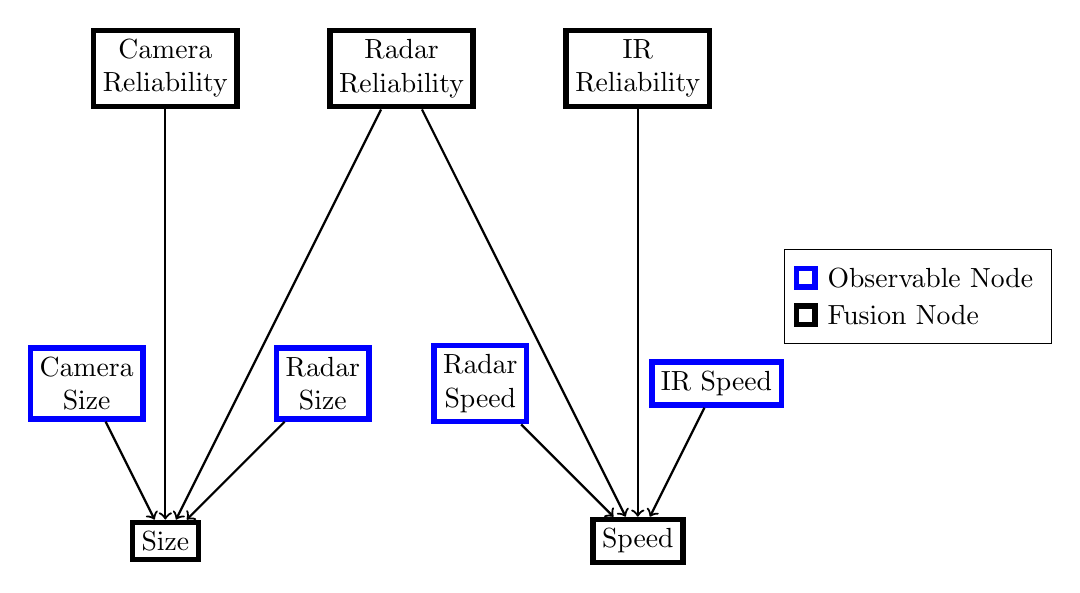
\begin{tikzpicture}[
  bluenode/.style={shape=rectangle, draw=blue, line width=2},
  blacknode/.style={shape=rectangle, draw=black, line width=2},
]
\path
(2,3) node[bluenode, align=center](c1){Camera\\ Size}
(5,3) node[bluenode, align=center](r2){Radar\\ Size}
(7,3) node[bluenode, align=center](r3){Radar\\ Speed}
(10,3) node[bluenode, align=center](i1){IR Speed}

(3,7) node[blacknode, align=center](c2){Camera\\ Reliability}
(6,7) node[blacknode, align=center](r4){Radar\\ Reliability}
(9,7) node[blacknode, align=center](i2){IR\\ Reliability}

(3,1) node[blacknode, align=center](s1){Size}
(9,1) node[blacknode, align=center](s2){Speed};



\draw[->, thick] (c1) -- (s1);
\draw[->, thick] (c2) -- (s1);
\draw[->, thick] (r4) -- (s1);
\draw[->, thick] (r4) -- (s2);
\draw[->, thick] (i2) -- (s2);
\draw[->, thick] (r2) -- (s1);
\draw[->, thick] (r3) -- (s2);
\draw[->, thick] (i1) -- (s2);

%Legend creation.
\matrix [draw, right] at (current bounding box.east) {
  \node [bluenode,label=right:Observable Node] {}; \\
  \node [blacknode, label=right:Fusion Node] {}; \\
};

\end{tikzpicture}
\end{center}
\caption{\label{fig:3_size_speed} Size and Speed input nodes and states.}
\end{figure}

\end{document}
